\documentclass[11pt,letterpaper]{article}
\usepackage{naaclhlt2016}
\usepackage{times}
\usepackage{latexsym}
\usepackage{color}

% More packages
\usepackage{amsmath}
\usepackage{amssymb}
\usepackage{framed}
\usepackage{graphicx}
%\usepackage{hyperref}
\usepackage{xspace}

% Some helpful macros
%% Abbreviations
\newcommand{\encdec}{\textsc{EncDec}\xspace}
\newcommand{\attn}{\textsc{AttnBaseline}\xspace}
\newcommand{\attncopy}{\textsc{AttnCopy}\xspace}
\newcommand{\atis}{\textsc{ATIS}\xspace}
\newcommand{\regex}{\textsc{Regex}\xspace}
\newcommand{\geo}{\textsc{Geo}\xspace}

\newcommand{\catroot}{\texttt{\$ROOT}\xspace}
\newcommand{\catquotstr}{\texttt{\$QuotStr}\xspace}
\newcommand{\catint}{\texttt{\$Int}\xspace}
\newcommand{\catstate}{\texttt{\$State}\xspace}
\newcommand{\catriver}{\texttt{\$River}\xspace}
\newcommand{\catcity}{\texttt{\$City}\xspace}

%% Mathematical Notation
\newcommand{\vocabin}{\mathcal{V}^{\text{(in)}}}
\newcommand{\phiin}{\phi^{\text{(in)}}}
\newcommand{\vocabout}{\mathcal{V}^{\text{(out)}}}
\newcommand{\phiout}{\phi^{\text{(out)}}}

%\naaclfinalcopy % Uncomment this line for the final submission
\def\naaclpaperid{***} %  Enter the naacl Paper ID here

% To expand the titlebox for more authors, uncomment
% below and set accordingly.
% \addtolength\titlebox{.5in}    

\newcommand\pl[1]{\textcolor{red}{[PL: #1]}}
\newcommand\rj[1]{\textcolor{blue}{[RJ: #1]}}

\newcommand\BibTeX{B{\sc ib}\TeX}


\title{Recurrent Neural Network Semantic Parsing
with Compositional Data Augmentation}
\author{Robin Jia\\
	    Computer Science Department\\
      Stanford University\\
	    {\tt robinjia@stanford.edu}
	  \And
    Percy Liang\\
    Computer Science Department\\
  	Stanford University\\
  {\tt pliang@cs.stanford.edu}}

\date{}

\begin{document}

\maketitle

\begin{abstract}
Current semantic parsers require complex machinery and
extensive feature engineering to achieve good performance.
Recurrent neural networks (RNNs)
have been shown to perform well at a wide range of sequence-to-sequence tasks.
In this work, we present a neural semantic parser
backed by a novel RNN model that allows the parser
to generalize to unseen entities.
In addition, we introduce the technique of
compositional data augmentation,
which helps our system to learn
about compositionality from limited amounts of training data.
Our system achieves good performance on a variety of semantic parsing tasks,
including new state-of-the-art numbers on the \regex domain.
\end{abstract}

\section{Introduction}
\begin{figure}[t] 
\small
\begin{center} 
  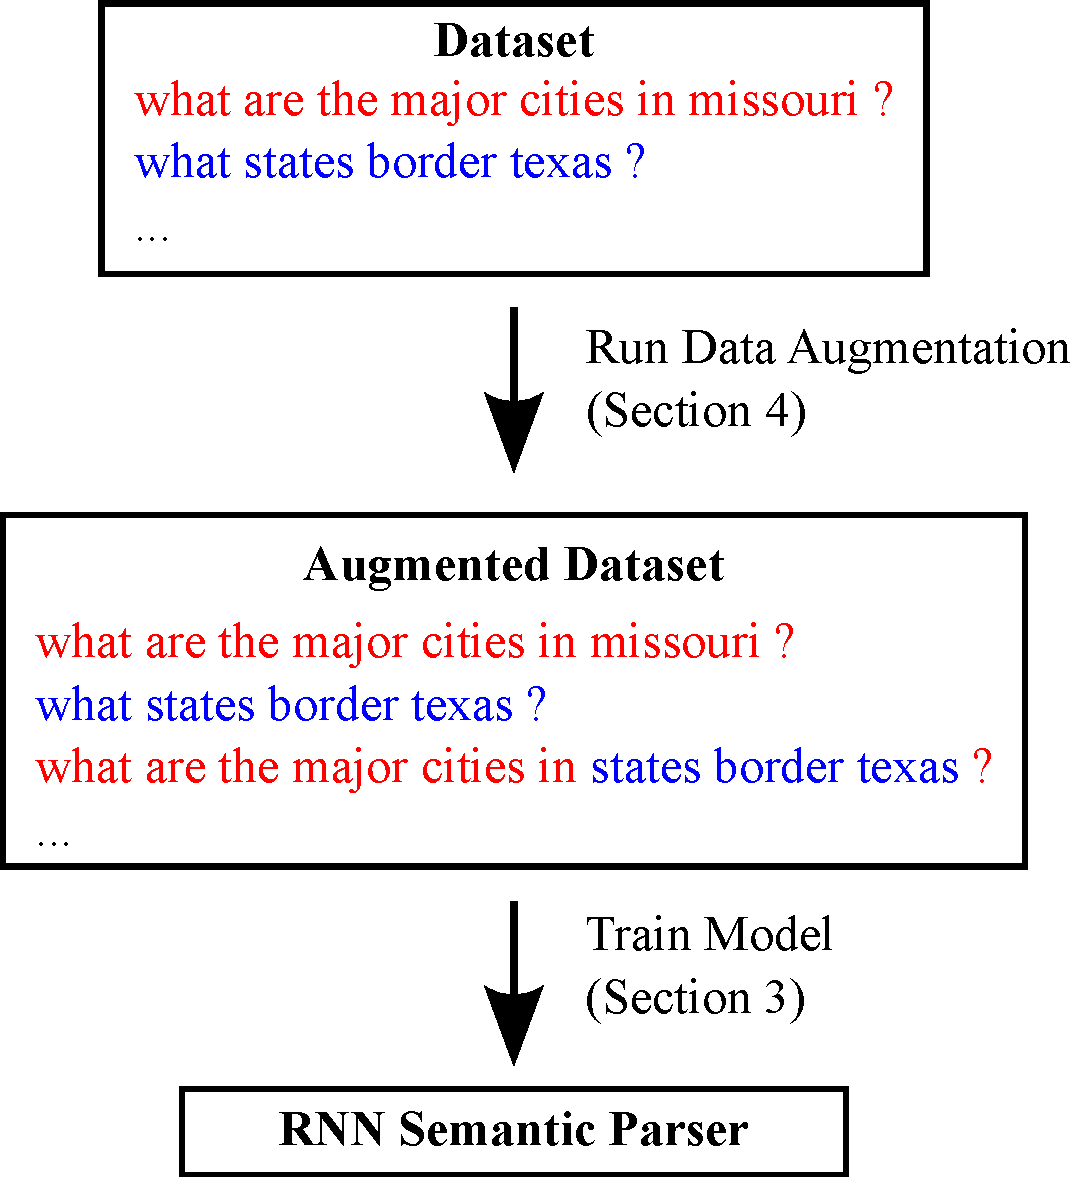
\includegraphics[scale=0.4]{fig-overview.pdf}
\end{center} 
\caption{An overview of our system.}
\label{fig:overview}
\end{figure}

Today, there exist a wide variety of applications that 
require semantic parsing--the precise translation of
natural language utterances into logical forms 
\cite{zelle96geoquery,zettlemoyer05ccg,zettlemoyer07relaxed,liang11dcs,artzi2013weakly,berant2013freebase,kushman2013regex}.
Modern semantic parsers are complex pieces of software
that require extensive hand-tuning and feature engineering.
Some recent work has tried to make semantic parsing
into a general purpose technology \cite{wang2015overnight},
but the performance of these systems leaves much to be desired.

Recently, recurrent neural networks (RNNs) have emerged
as a general-purpose technology for processing sequential data.
In particular, sequence-to-sequence RNN models
have achieved impressive results on a variety of natural language processing
tasks, including machine translation and syntactic parsing.
RNNs are also appealing for their simplicity, as they require 
little hand-engineering of features.

However, there are at least two significant barriers to applying these 
RNN models directly to semantic parsing.
First, semantic parsers are commonly trained from small datasets,
with possibly only hundreds of utterances paired with annotated logical forms.
At the same time, to perform well, semantic parsers
must be able to generalize to a large set of 
domain-specific entities which, due to the limited
amount of training data, may occur rarely or not at all
in the training dataset.
Second, most modern semantic parsing systems have built-in
prior knowledge about the compositional structure of language.
In contrast, RNNs can only learn about compositionality
through observations of the data.
With this paltry amount of supervision,
RNN models are in danger of severely overfitting the training data.

In this paper, we present the first (to our knowledge)
semantic parser that uses a sequence-to-sequence RNN model to generate
logical forms.  
Our contributions are twofold.
First, to address the issue of unseen entities,
we introduce a new RNN sequence-to-sequence model that uses 
attention to handle rare words.
Second, to prevent overfitting and teach the model about compositionality,
we introduce compositional data augmentation,
which induces a high-precision grammar from the given training data
and generates synthetic data by sampling from this grammar.

%\pl{
%Overall good - flows well and well-motivated, generally like the writing style.
%Currently, you do a good job of giving background about RNNs
%and the challenges that arise when applying to semnatic parsing.
%But the main thing that you need to do more of is highlight our contributions
%and connect it directly with challenges.
%Make it really crisp - don't go for subtlety here: for example,
%say there are two challenges, A, and B.  We tackle A using C and B using D.
%Make our contributions sound as exciting as the challenges!
%}


\section{Related Work}
Much excitement currently surrounds sequence-to-sequence RNNs.
Such models have been trained on such diverse tasks as
machine translation \cite{sutskever2014sequence,bahdanau2014neural}, 
syntactic parsing \cite{vinyals2015grammar}, and 
finding convex hulls \cite{vinyals2015pointer}, with impressive results on each.
%In particular, the recent work on syntactic parsing showed that
%even though RNNs are constrained to generate their output in a linear fashion,
%they can in fact learn to produce tree structures.

Nonetheless, there has yet to be a successful application of
neural networks for semantic parsing.
We are only aware of one previous effort 
by Grefenstette et al.~\shortcite{grefenstette2014deep},
though their model was not a sequence-to-sequence model,
and they had yet to achieve good results.

Current semantic parsing systems are complex pieces of software 
and have a great deal of prior knowledge baked into their internal structure.

\pl{need to argue the fact that current semantic parsers involve substantial
  work more convincingly and quantitatively;
  I don't think this is a fair comparison - but of the right flavor - number of lines
  of code in SEMPRE versus in nn-semparse
}

Data augmentation has been shown to help neural networks,
particularly in the field of computer vision.
AlexNet \cite{krizhevsky2012imagenet}, 
which at the time drastically improved
the state-of-art on ImageNet,
was trained on augmented data generated by applying various transformations
to the input images that did not change the output label.
The data augmentation scheme we propose has a more general flavor,
as it is not constrained to keep the output label fixed.
We are able to generate synthetic examples $(x, y)$
where both $x$ and $y$ are not seen in the training dataset.
% Another nice analysis (http://arxiv.org/pdf/1405.3531.pdf) 

\pl{I personally like putting the related work at the end with the discussion
we can get into more of an in-depth comparison and have more meaningful,
higher-level comparisions, rather than just being a cite-fest.
}

\section{Task}
We model semantic parsing as a generic sequence-to-sequence task.
The input utterance $x$ is tokenized into a sequence of words $x_1, \dotsc, x_m
\in \vocabin$, the input vocabulary;
similarly, the output logical form $y$ is tokenized
into a sequence of tokens $y_1, \dotsc, y_n \in \vocabout$, the output vocabulary.
Representing the logical form as a linear sequence of tokens
instead of an abstract syntax tree may seem unnatural,
but this choice makes it easier to define our RNN model.
Prior work on syntactic parsing 
\cite{vinyals2015grammar} has shown that
RNNs can indeed predict tree-strucutred outputs
when they are linearized in this fashion.

%\pl{this requires some brief discussion / justification: people
%naturally think of output sequence as tree structure.
%}

\pl{need FIGURE with a concrete example}

\subsection{Datasets}
\begin{table}[t]
  \centering
  \small
  \begin{tabular}{|l|c|c|c|}
    \hline
    Dataset & Training Examples & Test Examples \\
    \hline
    \geo & 600 & 280 \\
    \regex & - & - \\
    \hline
  \end{tabular}
  \caption{Overview of the datasets used in this paper.  
  For \geo, we use the standard 600/280 split first used by
  \protect\cite{zettlemoyer05ccg}.
  For \regex, we create our own split by randomly partitioning the dataset.}
  \label{tab:datasets}
\end{table}

We present results on a few different standard semantic parsing datasets.

\begin{itemize}
  \item \textbf{ATIS} (\atis).  The ATIS domain contains 
    natural language queries for an airplane flight database
    paired with corresponding database queries written in a 
    lambda calculus-based language.

  \item \textbf{Regular Expressions} (\regex).  The regular expressions domain
  contains natural language descriptions of regular expressions
  paired with associated regular expressions.

  \item \textbf{Geoquery} (\geo).  The geoquery domain
  contains natural language questions about US geography
  paired with corresponding database queries written in a prolog-based
  query language.
\end{itemize}

It is notable that these datasets are many orders of magnitude smaller
than the datasets used to train neural machine translation systems (CITE).
Similar work on syntactic parsing achieved good results
when trained on tens of thousands of parse trees.

In this work, we only explore learning from logical forms.
We therefore exclude some semantic parsing datasets
that only include denotations,
such as \textsc{WebQuestions} \cite{berant2013freebase}.
We discuss the possibility of learning from denotations
in the Discussion section.

%\pl{no intrinsic reason why we can't have denotations;
%state in a more neutral way}

\subsection{Implementation Details}
We tokenize logical forms in a domain-specific manner,
as this depends on the syntax of the formal language being used.
This tokenization is performed in such a way that
entity names can be easily copied from input to output.
At the same time, we intentionally perform name mangling on predicate names,
so that the model cannot cheat by copying these as well.
For example, in the \geo domain, we transform the name
of the predicate ``\texttt{city}'' to ``\texttt{\_city}''
so that the model cannot directly copy the word ``city'' from the input 
to output.

\section{Neural Semantic Parser}
Our neural semantic parser is based closely on existing
attention-based neural machine translation models.
In particular, we closely follow \cite{luong2015translation}.

At a high level, we can describe our system in terms of two main modules:
\begin{enumerate}
  \item \textbf{Encoder Module}.  This module 
    converts the input into a sequence of vectors,
    one per input token, that represent the input.
    It takes in the input sequence
    $x_1, \dotsc, x_m$ and generates a sequence of 
    annotations $b_1, \dotsc, b_m$,
    where each $b_i$ is a real-valued fixed-sized vector.
  \item \textbf{Decoder Module}.  This module
    takes in the input sequence and annotations,
    and generates a probability distribution
    over sequences $y = y_1, \dotsc, y_n$
    with elements in $\vocabout$.
\end{enumerate}
The decoder itself can be decomposed into three modules:
\begin{enumerate}
  \item \textbf{Decoder Initialization Module}.
    This module describes how to initialize the decoder.
    It takes in the annotations $b_1, \dotsc, b_m$, and
    outputs the initial decoder hidden state $s_0$,
    a real-valued vector.
  \item \textbf{Decoder Update Module}.  This module describes
    how to update the hidden state of the decoder.
    It module takes in the current decoder state $s_{j}$,
    the annotations $b_1, \dotsc, b_m$, and the most recently
    written token $y_{j+1}$, and outputs the new state $s_{j+1}$.
  \item \textbf{Decoder Ouptut Module}.  This module
    describes how the decoder generates the next token of the 
    output sequence.
    It takes in the current decoder hidden state $s_{j}$,
    the annotations $b_1, \dotsc, b_m$,
    and the original input sequence,
    and outputs a probability distribution 
    for $y_{j+1}$, the next word to write.
\end{enumerate}
In the next sections, we describe each of these modules in more detail.


%\pl{
%Think about good software engineering principles when you're defining the
%model.  What I mean is start by the abstract interfaces
%with modules Encode, Decode, etc.
%Define their types (sequence to vector, distribution over tokens, etc.)
%and give intuition about what they are supposed to do;
%forward reference the sections that talk about the modules.
%Absolutely don't just start jumping into model details.
%Start top-down.
%}

\pl{
  Also need at least one (probably two) figure(s)
  to illustrate (i) the abstract model framework,
  and (ii) a concrete example.  Use the same example as in Figure 1.
}

\subsection{Encoder Module}
The encoder module is a bi-directional LSTM, which we define
in more detail below.

First, each $x_i$ is mapped to a vector $\phiin(x_i)$.
Two RNNs--a forward RNN and a backward RNN--each take these vectors as input.
Each RNN starts with a fixed initial hidden state vector $h_0$, and 
generates a sequence of hidden states $h_1, \dotsc, h_m$ by
repeatedly applying the recurrence \[
  h_i = f(u_i, h_{i-1}),
\]
where $u_i$ is the word vector fed to the network at the $i$-th time step.
For the forward network, $u_i = \phiin(x_i)$; for the
backward network, $u_i = \phiin(x_{m-i})$, i.e. the sequence is read in reverse order.
In this work, we choose $f$ to have the form of an LSTM \cite{hochreiter1997lstm}.

Finally, we generate annotation vectors $b_i$ for each 
$i \in \{1, \dotsc, m\}$ by concatenating the 
state vector at time $i$ for the forward RNN and time $m-i$ 
for the backward RNN.  
In other words, $b_i$ is the concatenation of the forward
and backward hidden states that were generated
right after $\phi(x_i)$ was fed into the RNN.

\subsection{Decoder Initialization Module}
The decoder's initial state $s_0$ is computed from 
the concatenation of the final states of the two encoder RNNs.
In particular, if we let $h$ denote the
concatenation of the final states of the two encoder RNNs, then
\[
  s_0 = \tanh(W^{(i)} h)
\]
for some parameter matrix $W^{(i)}$.

\subsection{Decoder Update Module}
Now, we describe the decoder update module.
Like the encoder, the decoder has a function $\phiout$
that maps words in $\vocabout$ to vectors.

Our decoder uses an attention model similar to that of 
Luong et al.~\shortcite{luong2015translation}.
Given the current hidden state $s_j$, our model computes
a context vector $c_j$ as a weighted average of the annotation vectors
computed by the encoder.
This computation begins by computing a score for each input word $e_{ij}$ 
for $i \in \{1, \dotsc, m\}$, according to
\[
  e_{ij} = s_{j}^T W^{(u)} b_i
\]
for some parameter matrix $W^{(u)}$.
These scores are normalized to a probability by a softmax, producing \[
  \alpha_{ij} = \frac{\exp(e_{ij})}{\sum_{i=1}^m \exp(e_{ij})}.
\]
Finally, the context vector is computed as a weighted average of annotations: \[
  c_j = \sum_{i=1}^m \alpha_{ij} b_i.
\]
The state is updated according to the recurrence \[
  s_{j+1} = g(v_{j+1}, s_{j}),
\]
where $v_j$ is the concatenation of $\phiout(y_{j+1})$ and $c_{j}$.
The function $g$ is also in the LSTM family.
This method of treating the context vectors as part of the
input to the LSTM is called the ``input-feeding approach''
by Luong et al.~\shortcite{luong2015translation}.

\subsection{Decoder Output Module}
We describe two decoder output modules: a baseline module, and a
more sophisticated module that performs attention-based copying.

\subsubsection{Baseline}
\label{sec:baseline-output}
The baseline output module uses a simple softmax over all
output vocabulary words.
The probability of outputting word $w \in \vocabout$ at time $j$ is \[
  P(y_{j+1} = w \mid x, y_{1:j}) \propto \exp(U_{w}^T s_j),
\]
where $U$ is a matrix with rows indexed by elements of $\vocabout$.

\subsubsection{Attention-based Copying}
Semantic parsers must be able to handle a large set of entity names,
including ones that were not seen at training time.
Often times, these entity names
can be copied directly from the input to the output.
This observation motivates our attention-based copying output module.
We allow the network to copy a word directly from input to output,
with probability determined by the amount of attention paid to that input word.
More formally, we have
\begin{align*}
  P(y_{j+1} &= w \mid x, y_{1:j}) \propto 
  \\ &\exp(U_{w}^T s_j)
  + \sum_{i=1}^m \mathbb{I}[x_i = w] \exp(e_{ij}),
\end{align*}
where $e_{ij}$ is the attention score computed by the decoder update module.

We note that our attention-based copying can be seen as a 
combination of a standard softmax output layer
and a Pointer Network \cite{vinyals2015pointer}.  In a Pointer Network,
the only way to generate output is to copy a symbol from the input,
using an attention mechanism.

\subsection{Learning}
During training, we maximize loglikelihood of the correct
logical form.
This strategy differs from some other semantic parsing systems
(e.g. SEMPRE), which maximize loglikelihood of the correct
denotation.
We train the model using simple stochastic gradient descent.
Gradients are computed automatically using Theano \cite{bergstra2010theano}.

\pl{
  At some point, should contrast with existing semantic parsing systems
  which are heavily constrained by the grammar, whereas everything here is soft.
  Pros and cons?
}

\section{Compositional Data Augmentation}
The strength of deep learning models lies in their flexibility;
as discussed earlier, previous work has shown that
RNN sequence-to-sequence models in particular can be trained
to perform a wide variety of tasks.  
However, this flexibility also presents a challenge:
as these neural models have no preconceived notions,
they are at a disadvantage compared to specialized systems
that have domain knowledge baked in.
This challenge is a bigger issue in domains like semantic parsing
that have small training datasets, as
it may be difficult to discover the desired domain knowledge
from the data alone.

Our solution to this problem is to
augment the original training datasets with synthetic examples.
This approach allows us to inject prior knowledge into our system,
as the synthetic examples can be generated 
in a way that leverages domain knowledge.
Furthermore, we can continue to use a flexible, domain-general neural model.

For semantic parsing, one important phenomenon to model is compositionality.
We therefore use a \emph{compositional data augmentation} scheme
based on grammar induction.
We use the existing training examples to induce a
synchronous context-free grammar (SCFG) over utterances and logical forms.
We then generate new examples from this grammar,
and add these to our original training dataset.

We apply compositional data augmentation to both the \regex and \geo domains,
using a different grammar for each.
We describe our approach for each domain in more detail below.

%For example, the Washington SPF (CITE), 
%which uses combinatory categorial grammar (CCG),
%closely models the alignment between words in the utterance 
%and predicates in the logical form, as well as how these parts
%combine.  SEMPRE \cite{berant2013freebase} similarly builds up logical forms
%recursively from smaller sub-units.  In contrast,
%our neural semantic parser generates logical forms in a linear fashion,
%left-to-right.  It has no prior expectation that language should
%exhibit compositionality.

\pl{need an example / FIGURE illustrating compositionality - this is too abstract
}

\pl{This section to be written with more gravity / authority,
  and make it seem like the data augmentation that we're doing is \textbf{a thing}
  based on principles, not just some random thing we made up.
  Spend more time talking about the general procedure,
  and less time on the nitty-gritty of Regex and Geo,
  which are kind of boring.
}


\subsection{Augmentation for \regex}
\begin{figure}[t] 
\small
\begin{framed}
\footnotesize
\subsubsection*{Basic Rules}
\catint $\to (0, 0) \mid (1, 1) \mid \dotsb \mid (9, 9)$

\subsubsection*{Induced Rules}
Example: (``lines beginning with `Therefore' '', \texttt{"Therefore.*"})\\
Induced rules:

\quad \catroot $\to$ (``lines beginning with ` \catquotstr ' '', \texttt{"}\catquotstr\texttt{.*"})

\quad \catquotstr $\to$ (``therefore'', \texttt{"therefore"}) \\

Example: (``lines using more than 4 characters'', \texttt{".*.\{5,\}.*"})\\
Induced rules:

\quad \catroot $\to$ (``lines using more than \catint characters'', \texttt{".*.\{(\catint + 1),\}.*"})

\subsubsection*{Generated Examples} 
(``lines beginning with `free' '', \texttt{"free.*"})

(``lines using more than 6 characters'', \texttt{".*.\{7,\}.*"})

\dots
\end{framed}
\caption{Data augmentation on \regex.}
\label{fig:augment-regex}
\end{figure}

For \regex, our basic strategy is to find small pieces of 
utterances and regular expressions that we can align with high confidence.
We write two rules that capture the primary cases:
\begin{itemize}
  \item Quoted strings.  If a string appears inside quotation marks
    in the utterance, and is found verbatim in the corresponding
    regular expression, we assume that these align directly.
  \item Integers.  If exactly one integer occurs in both the 
    utterance and regular expression, we assume they should be aligned.
    If the integers are not equal, we assume that there should be
    a constant difference between them 
    (see Figure \ref{fig:augment-regex} for an example).
\end{itemize}

Our grammar therefore has three categories: 
\texttt{\$ROOT}, \texttt{\$QuotedStr}, and \texttt{\$Int}.
Figure \ref{fig:augment-regex}
provides more detail about data augmentation on \regex.

\subsection{Augmentation for \geo}
\begin{figure}[t] 
\small
\begin{framed}
\footnotesize
\subsubsection*{Induced Rules}
Example: ``what is the highest mountain in alaska ?''\\
Induced rules:

\quad \catroot $\to$ ``what is the highest mountain in \catstate ''\\

Example: ``what is the state with the lowest population ?''\\
Induced rules:

\quad \catstate $\to$ ``state with the lowest population''\\

Example: ``what river runs through illinois ?''\\
Induced rules:

\quad \catroot $\to$ ``what river runs through \catstate ?''

\quad \catriver $\to$ ``river runs through illinois''

\subsubsection*{Generated Examples} 
``what is the highest mountain in state with the lowest population ?'' \\
``what river runs through state with the lowest population ?'' \\
\dots
\end{framed}
\caption{Data augmentation on \geo.  Due to lack of space,
we only show the grammar over the natural language utterances.}
\label{fig:augment-geo}
\end{figure}

The \geo domain exhibits a greater degree of compositionality
than \regex, which presents an opportunity to use a more sophisticated
data augmentation strategy.
In particular, the more difficult \geo queries tend to have
nested sub-queries (e.g. ``states that border states that border colorado'').

To generate examples with multiple levels of nesting,
we induce a grammar that can combine two training examples into one.
We crucially leverage the fact that entity names are
easy to identify, and it is easy to align occurrences of entities
in the utterance and logical form.
Therefore, we can replace individual entity mentions
with entire phrases that evaluate to a set of entities of the same type.

We choose to focus on three types of entities--states, cities, 
and rivers--as they are the most common entity types in the dataset.
Therefore, our grammar has four categories:
\texttt{\$ROOT}, \texttt{\$State}, \texttt{\$City}, and \texttt{\$River}.
Figure \ref{fig:augment-geo}
provides more detail about data augmentation on \geo.

\section{Experiments}
We evaluate our system on three domains: \atis, \regex, and \geo.
For the \atis domain, we report exact logical form match accuracy.
For \regex, we determine correctness of a predicted regular expression
by first converting it and the gold regular expression to
deterministic finite automata (DFAs).  We then call the regular expressions
equivalent if and only if corresponding automata are equivalent.
This procedure is guaranteed to call two regular expressions equivalent
if and only if they define the same regular language.
Finally, for \geo, we determine correctness based on denotation match.

We compare our full system with attention-based copying, \textbf{\attncopy}, 
to two related baselines:
\begin{itemize}
  \item \textbf{\encdec}.  An encoder-decoder LSTM model (no attention)
    that uses the baseline decoder output module.
  \item \textbf{\attn}.  The same as \attncopy, except with the baseline decoder
    output module described in section~\ref{sec:baseline-output}.
\end{itemize}
\pl{these models should probably be defined in the model section as you build up to our
real model}

\subsection{Implementation Details}
We ran all experiments with a hidden size of $400$ units,
and $100$-dimensional word embeddings.
We initialized all parameters uniformly at random 
within the interval $[-0.1, 0.1]$.
We used a simple learning rate schedule:
we first train the model for $25$ epochs at a learning rate of $0.1$,
then for $5$ more epochs with a learning rate of $0.05$,
and finally $5$ additional epochs with a learning rate of $0.025$.
For the \attncopy model, we replace word vectors for words
that occur only once in the training set 
with a universal \texttt{<unk>} word vector;
we do not do this for the baselines, as without the copying mechanism,
replacing rare words with \texttt{<unk>} hurts performance.

Another important hyperparameter for \regex and \geo is the
extent to which we perform data augmentation.
For \regex, we train on the original dataset,
plus all NUMBER examples generated by the integer-based scheme
and $1000$ randomly sampled new examples generated by the string-based scheme.
For \geo, we train on the original dataset,
plus $500$ randomly sampled new examples.
All hyperparameters were tuned by training on a subset of the
training set, and evaluating on the remaining examples.

At test time, we use beam search with beam size $K=10$.
We automatically balance missing right parentheses.
We then pick the highest-scoring parse 
that can be processed by our domain-specific
equivalence-checking routine without errors.
On \geo, this means we take the highest-scoring parse
that does not yield an executor error when the
corresponding denotation is computed;
on \regex, this means that no error is thrown when 
converting the regular expression to a DFA.

\subsection{Main Results}
\begin{table}[t]
  \centering
  \small
  \begin{tabular}{|l|c|c|c|}
    \hline
    & \atis & \regex & \geo \\
    \hline
    \textbf{Previous Work} & & & \\
    Zettlemoyer and Collins~\shortcite{zettlemoyer07relaxed} & $84.6\%$ & & \\
    Kushman and Barzilay~\shortcite{kushman2013regex} & & $65.5\%$ & \\
    Kwiatkowski et al.~\shortcite{kwiatkowski10ccg} & & & $88.9\%$ \\
    Liang et al.~\shortcite{liang11dcs} & & & $91.1\%$ \\
    \hline
    \textbf{Original Dataset} & & & \\
    \encdec & - & - & - \\
    \attn & - & - & - \\
    \attncopy & $78.3$ & $65.0$ & $75.0$ \\
    \hline
    \textbf{With Data Augmentation} & & & \\
    \encdec & & - & - \\
    \attn & & - & - \\
    \attncopy & & $79.0$ & $84.0$ \\
    \hline
  \end{tabular}
  \caption{Results.}
  \label{tab:results}
\end{table}

We compare our system to state-of-art results
achieved on all three datasets (first group of rows of Table \ref{tab:results}).
For \atis and \regex, we compare to just a single state-of-art system.
On \geo, we list both Liang et. al.~\shortcite{liang11dcs}
and Kwiatkowski et. al.~\shortcite{kwiatkowski10ccg}.
The former system achieved the higher accuracy,
but it also was given as input an extended lexicon that
provided prior information about alignments between 
English words and predicates.  We explicitly take
care to avoid including such prior knowledge in our system.

First, we evaluate our system trained on the original dataset alone,
and no new examples generated by our data augmentation approach.
Our results are summarized in the second section of Table \ref{tab:results}.
Note that even without data augmentation, we are able to nearly
match the state-of-art on the \regex dataset.
However, we lag significantly behind on \geo.

Next, we now rerun our system and all baselines on our
augmented training datasets.  These results are shown in the
third and final section of Table \ref{tab:results}.
With data augmentation, we achieve a new state-of-art level performance
on \regex, by a considerable margin.  We are also much more competitive
with state-of-art on \geo.

% RJ: Omitting this section for now.  The pictures don't look _that_ convincing
% I settled on using a large hidden state, which I think makes it
% less necessary to attend to exactly the right place.
% In particular, you see many instances where the network chooses to attend to the word
% after you would expect it to attend to.
% \subsection{Learning Compositionality via Alignments}

\subsection{Real vs. Augmented Data}
\begin{figure}[t] 
\small
\begin{center} 
  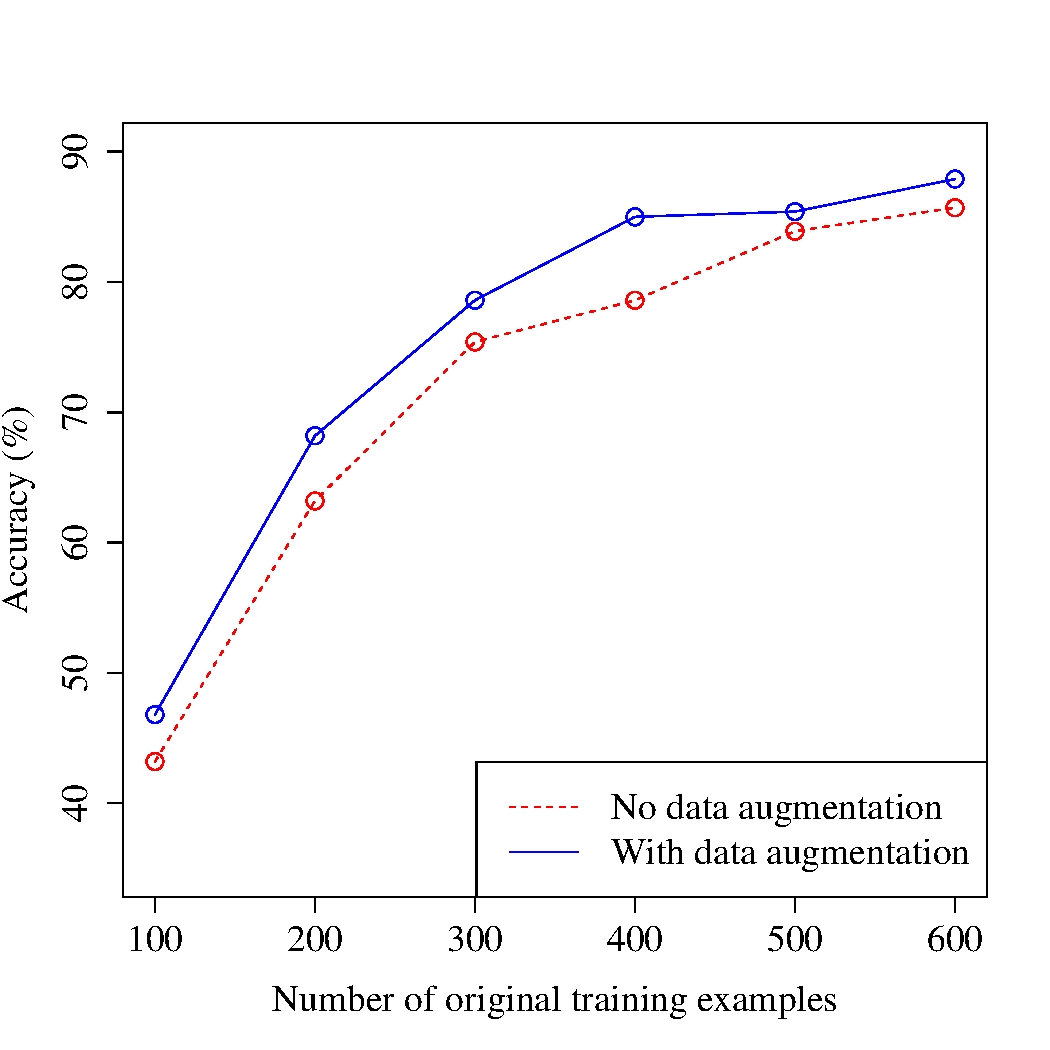
\includegraphics[scale=0.4]{fig-geo-augment.pdf}
\end{center} 
\caption{Accuracy on \geo as a function of number of training examples.
  Data augmentation gives a consistent performance boost,
regardless of original dataset size.}
\label{fig:geo-augment}
\end{figure}

We ran additional experiments on \geo to characterize
the extent to which data augmentation helps our system.
In particular, we wanted to compare the increase in performance
caused by adding synthetic data to the 
increase in performance caused by adding more actual examples.

In Figure~\ref{fig:geo-augment}, we plot dev accuracy as a function of
the number of real training examples.  The red line
shows results without data augmentation;
the blue line shows results when data augmentation was 
performed on the available training examples.
From this plot, we see that the effect of 
data augmentation is relatively constant regardless
of original training set size.
On the other hand, there are clear diminishing marginal returns
to adding real training examples, and the curve appears to level out
significantly below the curve for augmented data,
suggesting that the compositionally-generated data
provides a significant boost that could not be replicated
by annotating a few more examples.

\subsection{Experiments on Artificial Data}
% RJ: We can add more of these sorts of experiments, of course.
% These preliminary runs looked promising so I wrote this section.
\begin{table}[t]
  \centering
  \small
  \begin{tabular}{|l|c|}
    \hline
    Training Data & Accuracy (on Nested) \\
    \hline
    100 Nested (baseline) & $20.2\%$ \\
    100 Nested + 100 Simple & $91.4\%$ \\
    100 Nested + 100 Union & $95.0\%$ \\
    200 Nested & $97.2\%$ \\
    \hline
  \end{tabular}
  \caption{Results of the experiments on artificial data.}
  \label{tab:artificial}
\end{table}

To further understand the effects of compositional data augmentation,
we conducted additional experiments on artificial data.
The main question we wished to investigate was whether
data augmentation can be beneficial even if the examples generated
do not match that of the test distribution.
When a dataset is augmented in this fashion, we refer to it
as \emph{out-of-domain} data augmentation.

To this end, we generated synthetic examples from a simple grammar.
Each example is a pair $(x, y)$, where
$x$ is an english-like utterance and $y$ is a corresponding
logical form written in a variant of lambda-DCS \cite{liang2013lambdadcs}.
Our world contains a set of entities and a set of binary relations
on entities; we can think of entities as people
and the relations as relationships between two people, such as ``are friends,''
``are neighbors,'' etc.  
We generate the following sets of synthetic examples:
\begin{itemize}
  \item \textbf{Simple}: One relation and one entity, 
    e.g. ``friends of alice.''
  \item \textbf{Nested}: Two relations nested and one entity, 
    e.g. ``neighbors of friends of alice.''
  \item \textbf{Union}: One relation and the disjunction of two entities,
    e.g. ``friends of alice or bob.''
\end{itemize} 
We train our semantic parser to map utterances to logical forms,
varying the source of training data.
We evaluate on $500$ examples of the ``Nested'' variety.

To test our hypothesis that training examples that do not resemble
the examples at test time can still help the system learn,
we try training the model with examples drawn from the other two sets.
The results of our experiments are in Table~\ref{tab:artificial}.
We see that these out-of-domain examples
do help test-time performance greatly.

We can conclude from these experiments that there are many regimes
in which data augmentation can be helpful.
Clearly, if we augment the training dataset with examples that
are very similar to the test examples, we should expect performance to increase.
Furthermore, even if the synthetic examples are not that similar
to the test examples, they can still be beneficial.

It is interesting to compare this out-of-domain data augmentation
to multitask learning.
In multitask learning, a model is made to predict multiple outputs for a given input.
Even if one only cares about one of these outputs,
multitask learning can be helpful because it can act as a regularizer,
forcing the model to learn intermediate representations that generalize
better (TODO: find citations, I'm not actually sure how I know this).
Similarly, out-of-domain data augmentation may encourage
the model to learn better representations.

TODO: Also talk about covariate shift, find an artificial
setting where the covariate shift issue dominates.

%\subsection{Data Augmentation and Covariate Shift}
%\begin{table*}[t]
%  \centering
%  \small
%  \begin{tabular}{|l|c|c|c|}
%    \hline
%    Dataset & Accuracy & Accuracy on Int Examples & Accuracy on String Examples \\
%    \hline
%    Original & $65.0$ & $11/19$ & $54/82$ \\
%    Int-Augmented & $67.0$ & $15/19$ & $52/82$ \\
%    String-Augmented & $65.0$ & $8/19$ & $56/82$\\
%    All Augmented & $79.0$ & $17/19$ & $62/82$ \\
%    \hline
%  \end{tabular}
%  \caption{Performance on \regex using different data augmentation strategies.}
%  \label{tab:regex-shift}
%\end{table*}
%
%We have shown that data augmentation can yield significant improvements
%for our model, as it encourages the model to learn good alignments,
%a simple form of compositionality.  Nonetheless,
%there are also drawbacks to our data augmentation, as it introduces
%covariate shift: certain types of examples are more likely than others
%to occur in our augmented data.
%
%To illustrate the effects of covariate shift, we ran an additional
%experiment on the \regex dataset.  We trained our model
%on the original dataset plus augmented data generated only from the
%integer-based scheme; we also trained a separate copy of the model
%on the original dataset plus augmented data generated only from the
%string-based scheme.  
%
%The results of this experiment are summarized in Table \ref{tab:regex-shift}.
%We see that in isolation, each individual data augmentation scheme
%does not significantly help accuracy.
%The integer-based augmentation helps the model deal better
%with utterances that contain an integer 
%(third column of Table \ref{tab:regex-shift}),
%but hurts performance on other examples.
%Similarly, the string-based augmentation helps the model
%deal better with utterances that contain quoted strings 
%(fourth column of Table \ref{tab:regex-shift}),
%but hurts performance on other examples.
%Pooling both sources of augmented data improves performance
%across the board.

\pl{I think we need to have more explicit top-down text saying what we're
  trying to accomplish from these experiments, and what we learned.  You do
  this to some extent already - just need more.
  Maybe the problem is that there's just a lot of boring experimental detail/setup
  that kind of gets in the way, and maybe can be compartmentalized more.
}

\pl{
  Try to connect the experiments more directly with our contributions / claims
  / intuitions that we built up over the course of the paper.
  We have a new model - ok - does it help?
  We have a new data augmentation scheme - does it help?
  etc.
}

\section{Discussion}
In this paper, we have presented the first RNN sequence-to-seqeunce
model for semantic parsing.  Our model is easy to train
and gives good performance on a wide variety of semantic parsing
datasets, when trained with logical form supervision.
Additionally, we describe a compositional data augmentation approach that 
further boosts performance.

While our data augmentation techniques are effective,
they unfortunately require non-trivial manual processing.
One line of potential future work would be to
perform data augmentation using a grammar
that was induced automatically, in a domain-general manner.
We could leverage existing work on semantic parsing
using higher-order unification \cite{kwiatkowski10ccg}.

One limitation of our current approach is that it 
requires annotated logical forms.
In the last few years, there has been an emergence of
semantic parsers that can learn from denotations 
\cite{liang11dcs,berant2013freebase}.
Such systems have a built-in understanding of the space of
syntactically valid logical forms, which our RNN semantic parser lacks.
In order to train our system from denotation information alone,
we would need to somehow teach it this information ahead of time.
Building on the data augmentation described in this paper,
we could use synthetic data with logical form supervision
to teach our system about the logical language.
For example, we could generate
pairs of ``canonical'' utterances and logical forms,
as in \cite{wang2015overnight}.  
We would first train the system to map
canonical utterances to logical forms, so that it would learn to produce
valid logical forms that are related to the input;
then, we could add in more data that pairs real utterances with denotations.

An alternative direction would be to incorporate the execution
step iself into the network.  Yin et al.~\shortcite{yin2015enquirer}
explore the idea of having a neural network that maps
SQL queries to denotations.  Such a system could be trained
on natural language queries instead of SQL.
Another piece of work in this vein is 
that of Bordes et al.~\shortcite{bordes2015simple}.
They similarly replace a database engine with a memory network
whose memories encode all the relations in the database.

\section*{Acknowledgments}
Do not number the acknowledgment section.

\section*{Reproducibility}
All experiments will be available on 
%\url{http://www.codalab.org}

\bibliography{all}
\bibliographystyle{naaclhlt2016}


\end{document}
